\documentclass{beamer}
\usetheme{default}
\usecolortheme{default}

\setbeamertemplate{navigation symbols}{}
\setbeamertemplate{footline}[page number]
\setbeamertemplate{caption}[numbered]
\setbeamertemplate{itemize items}[circle]
\setbeamertemplate{enumerate items}[square]
\setbeamercolor{footnote mark}{fg = red}

\usepackage [T2A] {fontenc}
\usepackage [utf8] {inputenc}
\usepackage [english, russian] {babel}
\usepackage{graphicx}

\title{Пространственно локализованные решения уравнения Гросса--Питаевского с переодически модулированной нелинейностью}

\author{Лебедев М. Е.}
\institute{
	Институт математики с вычислительным центром \\ УФИЦ РАН \\
	\medskip
	\textit{gloriouslair@gmail.com}
}
\date{Декабрь \\ 2020}

\begin{document}

% ************
% * SLIDE 01 *
% ************
\begin{frame}
	\titlepage
\end{frame}

% ************
% * SLIDE 02 *
% ************
\begin{frame}
	\frametitle{Модель}
	
	Одномерное уравнение Гросса--Питаевского:
	\begin{equation}
		i\Psi_t + \Psi_{xx} - U(x) \Psi + P(x) |\Psi|^2 \Psi = 0, \quad U(x), P(x) \in \mathbb{R};
		\label{eq:initial}
	\end{equation}
	
	\begin{block}{В контексте теории БЭК\footnotemark[1]:}
		\begin{itemize}
			\item $\Psi(t, x)$ --- макроскопическая волновая функция конденсата;
			\item $U(x)$ --- линейный потенциал ловушки; % ловушка, удерживающая конденсат
			\item $P(x)$ --- нелинейный потенциал, характеризует межатомное взаимодействие (притяжение $+$ / отталкивание $-$).
		\end{itemize}
	\end{block}
	
	{\it Стационарные решения}: $\Psi(t, x) = u(x) e^{-i \omega t}$.

	\begin{equation}
		u_{xx} + Q(x) u + P(x) u^3 = 0, \quad Q(x) = \omega - U(x)
		\label{eq:stationary}
	\end{equation}
	
	\footnotetext[1]{\footnotesize{Y.V. Kartashov, B.A. Malomed, L. Torner Solitons in nonlinear lattices // Rev. Mod. Phys. 2011. 83. P.247–305.}}
\end{frame}

% ************
% * SLIDE 03 *
% ************
\begin{frame}
	\frametitle{Определения}
	
	\begin{block}{Локализованное решение}
		$\lim \limits_{x \to \pm \infty} u(x) = 0.$
	\end{block}

	\begin{block}{Сингулярное решение}
		$\exists x_0, \lim \limits_{x \to x_0} u(x) = \infty$.	
	\end{block}

	\begin{block}{Регулярное решение}
		Не является сингулярным.
	\end{block}

	\begin{block}{Устройчивое решение}
		Достаточно малое возмущение не возрастает со временем.	
	\end{block}

\end{frame}

% ************
% * SLIDE 04 *
% ************
\begin{frame}
	\frametitle{Задача}
	
	Выяснить влияние периодического нелинейного потенциала $P(x)$ на структуру семейства стационарных локализованных решений уравнения \eqref{eq:initial} и их устойчивость.
	
	% Указать также более конкретные задачи
\end{frame}

% ************
% * SLIDE 05 *
% ************
\begin{frame}
	\frametitle{Утверждения о регулярных и сингулярных решениях}

	\begin{block}{Утверждение 1}
		Пусть $\forall x \in \mathbb{R}$, функции $Q(x)$, $P(x) \in C^1(\mathbb{R})$, причем $P(x) > 0$, $Q(x) \ge Q_0~(\exists Q_0)$, тогда все решения задачи Коши для уравнения (\ref{eq:stationary}) c произвольными НУ $(u_0, u_0')$ {\bf регулярны}\footnotemark[2]. 
	\end{block}

	\begin{block}{Утверждение 2}
		Пусть $\forall x \in \mathbb{R}$ выполняются условия: $P(x) < 0$, $Q(x) < 0$, тогда все решения уравнения (\ref{eq:stationary}) {\bf сингулярны}, за исключением нулевого решения\footnotemark[2].
	\end{block}

	\begin{block}{Утверждение 3}
		Пусть $P(x) <> 0$ (не знакоопределена); $\exists x_0$, $P(x_0) < 0$, тогда при некоторых ограничениях на $Q(x)$, $P(x)$ существуют два $C^1$~--~гладких однопараметрических семейства решений уравнения (\ref{eq:stationary}) {\bf сингулярных} в точке $x_0$\footnotemark[2].
	\end{block}

	\footnotetext[2]{\footnotesize{G. L. Alfimov, M. E. Lebedev, Ufa Mathematical Journal. Vol. 7. No. 2 (2015). P. 3-17.}}
\end{frame}

% ************
% * SLIDE 06 *
% ************
%\begin{frame}
% 	\frametitle{Утверждения о регулярных и сингулярных решениях}
%	\framesubtitle{Асимптотические разложения для семейств коллапсирующих решений}
%\end{frame}

% ************
% * SLIDE 07 *
% ************
\begin{frame}
	\frametitle{Классификация}
	\framesubtitle{Основания}
	
	\begin{itemize}
		\item $U(x) \equiv 0$, линейный потенциал отсутствует;
		\item $P(x + L) = P(x)$, периодический нелинейный потенциал;
		\item $P(x) <> 0$, сингулярность --- типичное поведение решений;
		\item $\omega < 0$, наличие локализованных решений.
	\end{itemize}
	
	\begin{equation}
		u_{xx} + \omega u + P(x) u^3 = 0.
		\label{eq:classification}
	\end{equation}
	
	\medskip
	
	Если <<большая часть>> решений уходит на бесконечность, тогда множество регулярных решений может быть описано в терминах символической динамики\footnotemark[3].
	
	\footnotetext[3]{\footnotesize{G. L. Alfimov, A. I. Avramenko, Physica D 254, 29 (2013)}}
\end{frame}

% ************
% * SLIDE 08 *
% ************
\begin{frame}
	\frametitle{Классификация}
	\framesubtitle{Аппарат}

	\begin{block}{Множества $\mathcal{U}_L^{\pm}$}
	$\mathcal{U}_L^{\pm} = \{ (u_0, u_0') \in \mathbb{R}^2$ | решение задачи Коши для уравнения \eqref{eq:classification} с НУ $(u_0, u_0')$ не сингулярно на $[0, {\pm} L] \}$, $\mathcal{U}_L = \mathcal{U}_L^+ \cap \mathcal{U}_L^-$.
	\end{block}

	\begin{block}{Отображение Пуанкаре $\mathcal{P}: \mathbb{R}^2 \to \mathbb{R}^2$}
		$\mathcal{P} (u_0,u_0') = (u(L), u'(L))$, где $u(x)$ --- решение с НУ $(u_0, u_0')$.
	\end{block}

	\begin{block}{Орбита}
		Последовательность точек $\{ p_n \}$ таких, что $\mathcal{P}(p_n) = p_{n+1}$.
	\end{block}

	\begin{block}{$\Sigma: \mathcal{O} \to \Omega^N$}
		Можно определить соответствие ($\Sigma$) между {\it орбитами} регулярных решений ($\mathcal{O}$) и {\it последовательностями} над алфавитом из $N$ символов ($\Omega^N$), где каждый символ соответствует компоненте связности множества $\mathcal{U}_L$.
	\end{block}
\end{frame}

% ************
% * SLIDE 09 *
% ************
\begin{frame}
	\frametitle{Классификация}
	\framesubtitle{Пример множеств $\mathcal{U}_L^{\pm}$}
	$$P(x) = \alpha + \cos{2x}, \quad \alpha \in (-1; +1)$$
	\begin{figure}
		\center{\includegraphics[width=1\textwidth]{pic/sets.pdf}}
		\caption{Множества $\mathcal{U}_{\pi} = \mathcal{U}_{\pi}^+ \cap \mathcal{U}_{\pi}^-$ для различных значений $\omega$, $\alpha$}
		\label{pic:sets}
	\end{figure}
\end{frame}

% ************
% * SLIDE 10 *
% ************
\begin{frame}
	\frametitle{Классификация}
	\framesubtitle{Построение алфавита: $\omega = -1$, $\alpha = -0.1$}
	\begin{figure}
		\center{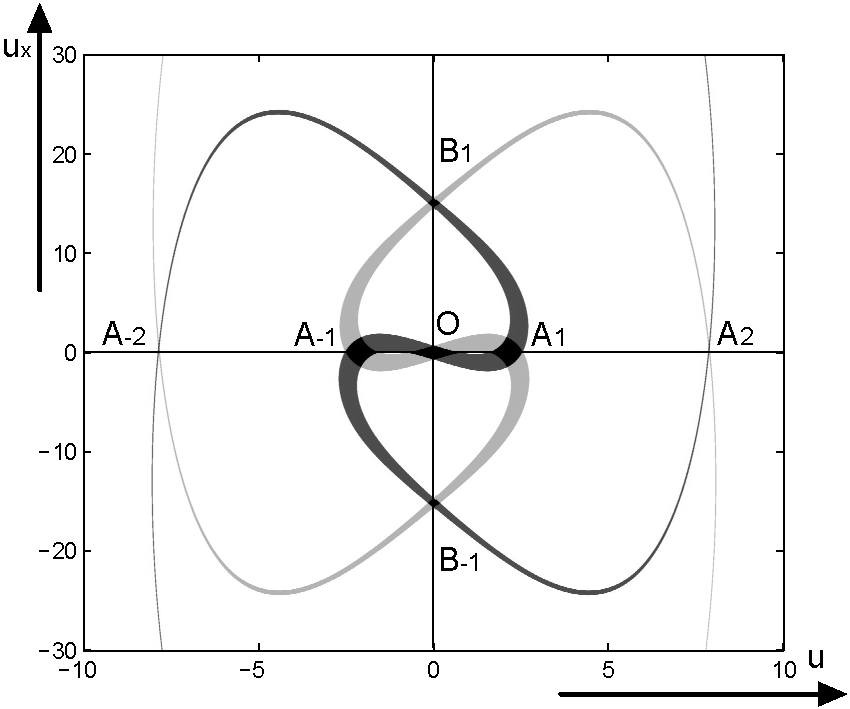
\includegraphics[width=0.75\textwidth]{pic/alphabet.pdf}}
		\caption{Спиралевидная структура $\mathcal{U}_{\pi}^{\pm}$ $\Rightarrow$ бесконечный алфавит.}
		\label{pic:alphabet}
	\end{figure}
\end{frame}

% ************
% * SLIDE 11 *
% ************
\begin{frame}
	\frametitle{Классификация}
	\framesubtitle{Кодировка решений}
	
	\begin{figure}
		\center{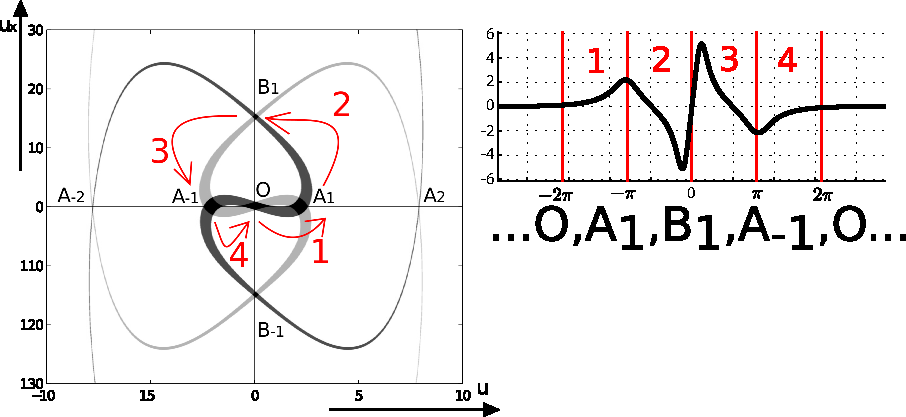
\includegraphics[width=1\textwidth]{pic/coding.pdf}}
		\caption{Пример построение кода для заданного решения}
		\label{pic:coding}
	\end{figure}
\end{frame}

% ************
% * SLIDE 11 *
% ************
\begin{frame}
	\frametitle{Классификация}
	\framesubtitle{Взаимно однозначное соответствие}
	
	Когда соответствие $\Sigma$ является взаимно однозначным?\footnotemark[3]
	\begin{enumerate}
		\item Множество $\mathcal{U}_L$ состоит из непересекающихся {\it островов}: $\mathcal{U}_L = \bigcup_{i \in S} D_i$.
		\item $\mathcal{P} D_i \cap D_j$, $\mathcal{P} D_i \cap D_j$ непусты; действие $\mathcal{P}$ на кривые внутри $D_i$ сохраняет свойства монотонности.
		\item $\Delta_0 = \mathcal{U}_L$, \quad $\Delta_{n + 1}^+ = \mathcal{P} \Delta_n^+ \cap \Delta_0$, \quad $\Delta_{n + 1}^- = \mathcal{P}^{-1} \Delta_n^- \cap \Delta_0$,\begin{center}
				$\lim \limits_{n \to \infty} \mu( \Delta_n^{\pm} ) = 0$.
			\end{center} 
	\end{enumerate}
	
	% Here could be some pictures, which clarify dynamics of the Poincare map on the phase plane.
	% Some h, v - strips could be depicted here.
	\begin{figure}
		\center{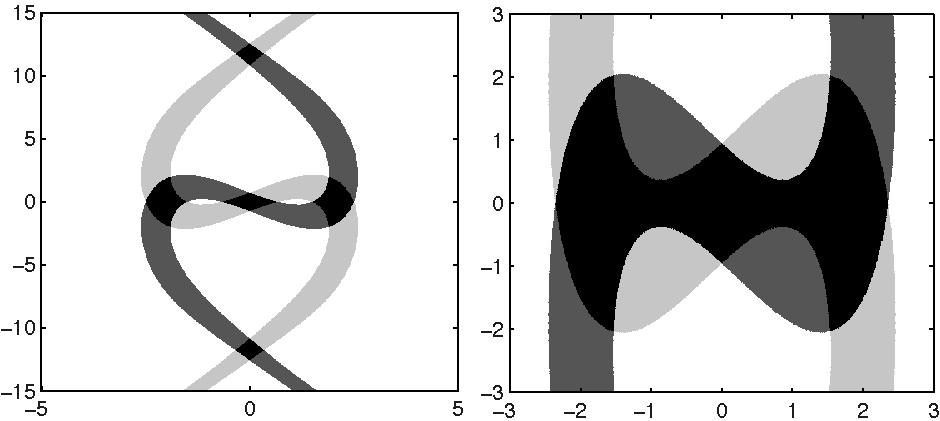
\includegraphics[width=0.5\textwidth]{pic/islands.pdf}}
		\caption{Пример островного и не островного множества $\mathcal{U}_{L}$}
		\label{pic:coding}
	\end{figure}
	
	\footnotetext[3]{\footnotesize{G. L. Alfimov, A. I. Avramenko, Physica D 254, 29 (2013)}}
\end{frame}

% ************
% * SLIDE 12 *
% ************
\begin{frame}	
	\begin{figure}
		\center{\includegraphics[width=0.9\textwidth]{pic/classification.pdf}} 
		\caption{Решения и их коды при $\omega = -1$, $\alpha = -0.1$}
		\label{pic:classification}
	\end{figure}
\end{frame}

% ************
% * SLIDE 13 *
% ************
\begin{frame}
	\frametitle{Устойчивость}
	\framesubtitle{\dots}	
\end{frame}

% ************
% * SLIDE XX *
% ************
\begin{frame}
	\begin{center}
		{\bf QA}
	\end{center}
\end{frame}

\end{document} 